\documentclass{beamer}
\usetheme{ucl}

\setbeamercolor{banner}{bg=darkblue}
\setbeamercolor{structure}{fg=black}

\setbeamersize{description width=2em}
\setbeamertemplate{navigation symbols}{\vspace{-2ex}}
\setbeamercolor{frametitle}{fg=white}

\title[Short Title]{Digital Implementation of End-to-End Machine Learning in Optical Communication System}
\author[Auth.1 \and Auth.2 \and Auth.3 \and Auth.4]{An Vo \\\and Mindaugas Jarmolovi\v{c}ius\\\and Oliver Jaison \\\and Tharmetharan Balendran}


\institute[UCL]{%
	Dept. of Electronic and Electrical Engineering \\ %
	University College London
}
\date{16th of May, 2021}

\begin{document}
	
	\frame{\titlepage}
	
	\begin{frame}
		\frametitle{Motivation}
		\begin{itemize}
		    \item Main focus of this project is studying end-to-end machine learning implementation in IM-DD optical communication networks
		    \item Aim to compensate for chromatic dispersion and non-linear photodiode detection allowing for longer feasible transmission distances
		    \item Main Objectives of this project:
		    \begin{itemize}
		        \item Simulating the Optical Channel
		        \item End-to-End Neural Network design and training
		        \item SystemVerilog Implementation of Neural Network
		    \end{itemize}
		\end{itemize}
	\end{frame}
	
	\begin{frame}
		\frametitle{Beautiful!!}
		This is some text in the first frame. This is some text in the first frame. This is some text in the first frame.
		
		\begin{center}
		    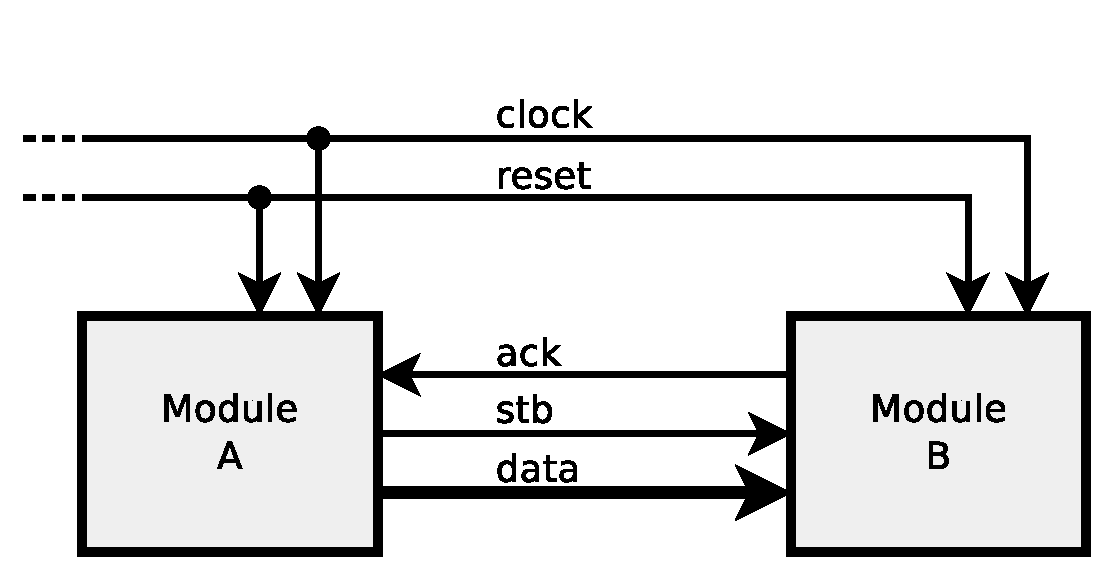
\includegraphics[width=0.7\textwidth]{resources/digital_circ/abus.eps}    
		\end{center}
		
	\end{frame}
	
	\begin{frame}
		\frametitle{Beautiful!!}
        \begin{alertblock}{Help!}
            text here
            \begin{itemize}
            \item point 1
            \end{itemize}
        \end{alertblock}
        
        \begin{block}{A block}
            An environment inside the block
            \begin{description}
            \item[The first step:] This is a very long description, and will wrap onto
              the next line
            \item[Step B:] text
            \end{description}
        
            \begin{itemize}
            \item a
            \item b
            \end{itemize}
          \end{block}
	\end{frame}
	
	
\begin{frame}
	\frametitle{An's Slide}
\end{frame}
	
\begin{frame}
	\frametitle{Min's Slide}
\end{frame}
	
\begin{frame}
	\frametitle{Oliver's Slide}
\end{frame}
	
\begin{frame}
	\frametitle{Tam's Slide}
\end{frame}
	
	\begin{frame}
	    \centering
		\huge{The End}
	\end{frame}
	
\end{document}